\section{Correlation Analysis}

Given the large number of features (338 in total), it was necessary to identify and remove features that are poorly correlated with
the target variable as well as those that are highly correlated with each other. Due to the high number of features, a visual approach,
such as a correlation matrix, was not feasible. Instead, two filters were applied to select the most
relevant features using the Spearman correlation coefficient, as the normality test failed.\\
The first filter is based on the correlation between the features and the target variable. Features with a correlation below a certain
threshold with the target variable are removed.\\
The second filter focuses on the correlation among the features themselves.
It counts, for each feature, the number of other features with which it has a correlation above a certain threshold. Features with a
number of correlations above a specified threshold are then removed.\\

\begin{algorithm}
    \caption{Feature Selection Process}
    \begin{algorithmic}[1]
        \State \textbf{Step 1:} Compute  the normal test (D'Agostino Pearson).
        \State \textbf{Step 2:} Compute the Spearman correlation coefficient for each feature with the target variable.
        \State \textbf{Step 3:} Apply the first filter to remove features with a correlation below a certain threshold with the target variable.
        \State \textbf{Step 4:} Compute the correlation matrix among all features.
        \State \textbf{Step 5:} Apply the second filter to remove features that have a high number of correlations (above a certain threshold)
        with other features.
        \State \textbf{Step 6:} Choose threshold values empirically and apply the filters using various combinations of these thresholds.
        \State \textbf{Step 7:} Train Random Forest models on the filtered data to evaluate performance and select the best combination of thresholds.
    \end{algorithmic}
\end{algorithm}

\subsection{Threshold Selection and Model Evaluation}

Threshold values were chosen empirically and the filters were applied using the combinations shown in Table \ref{tab:threshold_values}.
Using the filtered data, Random Forest models were trained and evaluated, as Random Forest was found to be the best performing model.
The optimal combination of thresholds was found to be: threshold 1 = 0, threshold 2 = 0.6 and number of features = 30, resulting in 30 features.

\rowcolors{2}{blue!8}{blue!18}
\begin{table}[h]
    \centering
    \small
    \begin{tabular}{|c|c|c|}
        \hline
        \textbf{Threshold} & \textbf{Values}                 \\
        THRESHOLD 1        & 0 - 0.1 - 0.2 - 0.3 - 0.4 - 0.5 \\
        THRESHOLD 2        & 0.6 - 0.7 - 0.8 - 0.9 - 1       \\
        N° FEATURES        & 5 - 10 - 15 - 20 - 25 - 30 - 40 \\
        \hline
    \end{tabular}
    \caption{threshold values}
    \label{tab:threshold_values}
\end{table}
\noindent
With threshold 1 = 0, the filter on the correlation between the features and the target variable was effectively bypassed.
However, with threshold 2 = 0.6, a stringent filter was applied on the correlation among the features themselves,
removing features that had a correlation above 0.6 with at least 30 other features. This indicates that having features
highly correlated with each other is more detrimental to the model than having features poorly correlated with the target variable.\\
Figure \ref{fig:comparison_model_on_all_features_vs_model_on_best} shows the results obtained with the model trained on filtered features
compared to the model trained on all features. As demonstrated, the model trained on filtered features performs significantly better.

\begin{figure}[H]
    \centering
    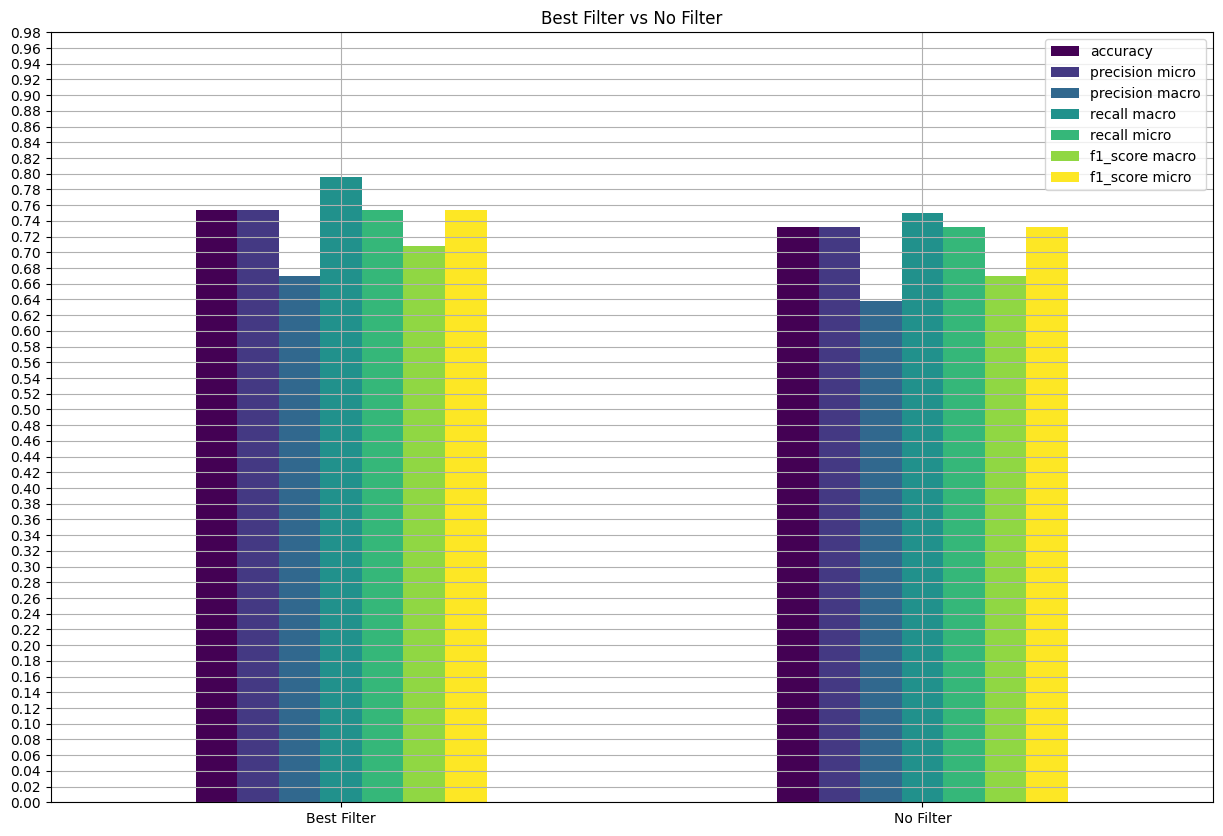
\includegraphics[width=0.8\columnwidth]{../images/model_on_all_features_vs_model_on_best.png}
    \caption{Comparison of different metrics between the model on all features and the model on the filtered ones}
    \label{fig:comparison_model_on_all_features_vs_model_on_best}
\end{figure}

\subsection{Selected Features and Correlation Matrix}

From this analysis, 41 features remained: 28 MFCC, 12 Chroma, and 1 ZCR.
The correlation matrix of the filtered features is shown in Figure \ref{fig:correlation_matrix}.
This matrix illustrates the pairwise correlation between the selected features, with the color intensity
indicating the strength and direction of the correlation. Dark red cells represent high positive correlations,
while dark blue cells indicate high negative correlations.

\begin{figure}[H]
    \centering
    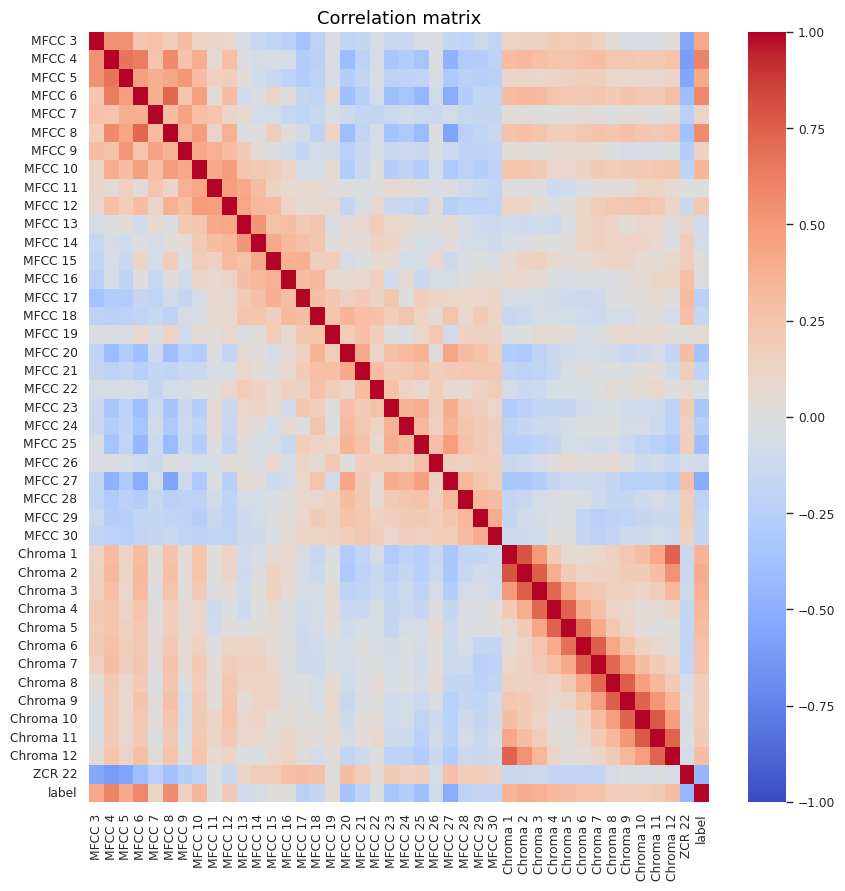
\includegraphics[width=0.8\columnwidth]{../images/correlation_matrix.png}
    \caption{Correlation matrix of the filtered features}
    \label{fig:correlation_matrix}
\end{figure}
\noindent
The matrix demonstrates that the remaining features have low correlations with each other, as evidenced by the predominantly
light colors away from the diagonal. This implies that the features are relatively uncorrelated, preventing multicollinearity
issues and enhancing the robustness of the model. The high diagonal values indicate that each feature is perfectly correlated
with itself, which is expected. However, the off-diagonal values being close to zero for most feature pairs confirm that the filtering
process was effective in selecting features that do not exhibit high inter-correlations.
